\section{\texorpdfstring{Program TIM2 s přerušením}{Program TIM2 s prerusenim}}

% =====================================================================================================================
	\begin{frame}
    \frametitle{Zadání}
		
		\begin{enumerate}
			\item Použijeme program pro \textbf{TIM2} z předchozí přednášky,
			\item upravíme hlavní smyčku tak, aby nevykonávala žádnou funkci,
			\item blikání LED přesuneme do obsluhy přerušení přetečení \textbf{TIM2},
			\item přerušení povolíme a zaregistrujeme na příslušném vektoru.
		\end{enumerate}	

	\end{frame}
	
% =====================================================================================================================
	\begin{frame}
    \frametitle{Povolení přerušení periferie}

		\begin{center}
			
\includegraphics[width=0.80\textwidth]{fig/tim2_navod.png}
		\end{center}
		
	\end{frame}
	
% =====================================================================================================================
	\begin{frame}
    \frametitle{Úprava definičních konstant}

		\begin{center}
			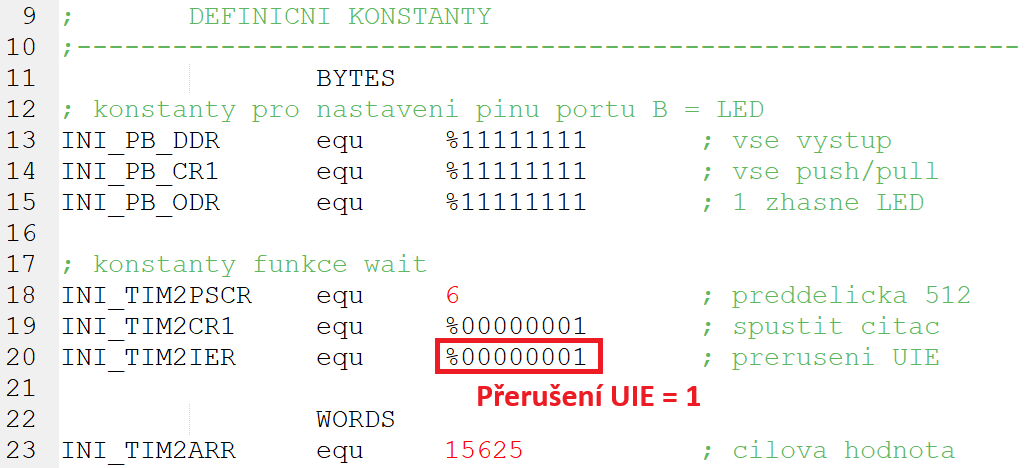
\includegraphics[width=0.90\textwidth]{fig/prg_tim2_definice.png}
		\end{center}
		
	\end{frame}
	
% =====================================================================================================================
	\begin{frame}
    \frametitle{Úprava programu}

		\begin{center}
			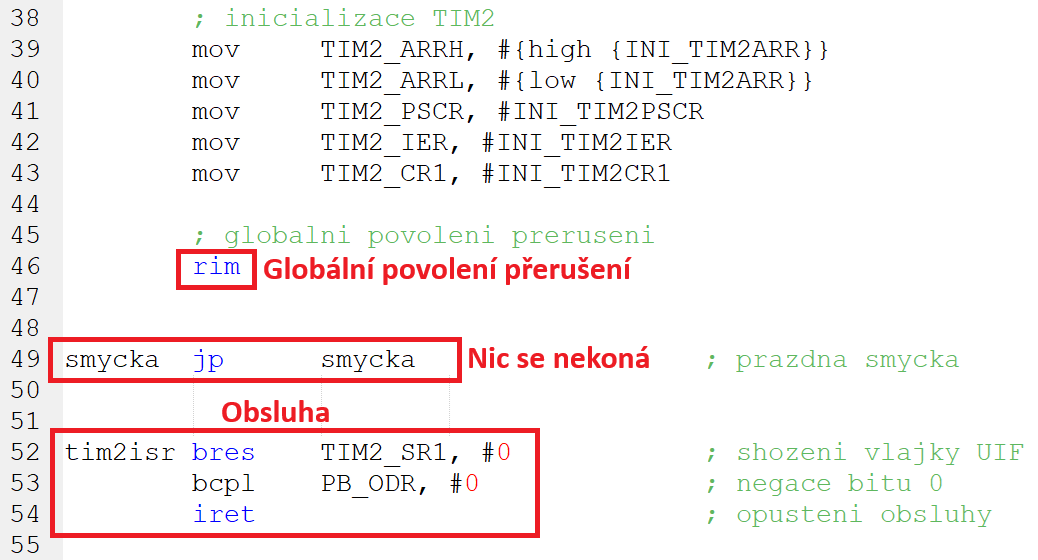
\includegraphics[width=0.90\textwidth]{fig/prg_tim2_smycka.png}
		\end{center}
		
	\end{frame}
	
% =====================================================================================================================
	\begin{frame}
    \frametitle{Zápis vektoru přerušení}

		\begin{center}
			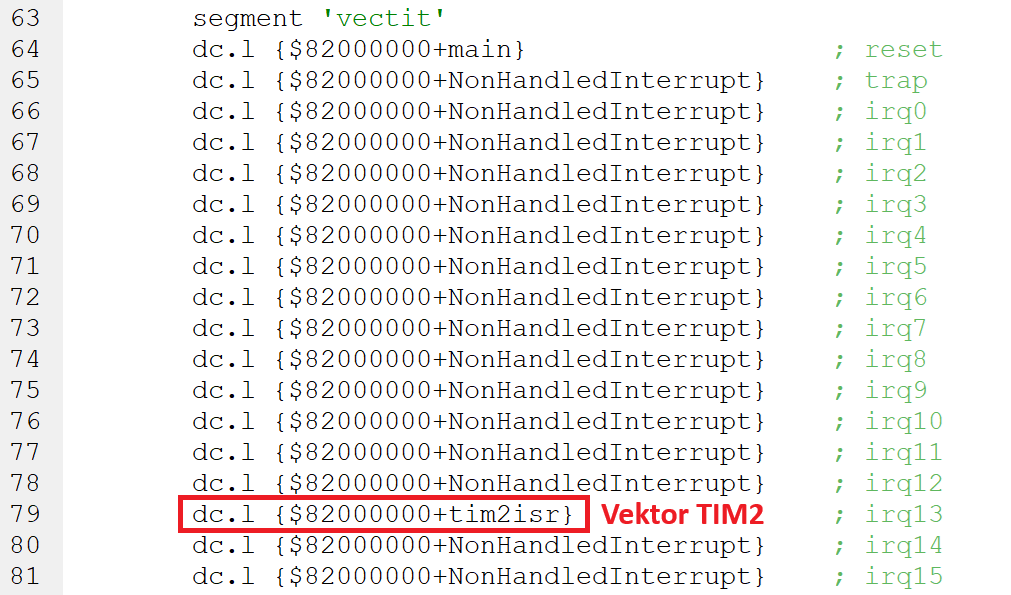
\includegraphics[width=0.90\textwidth]{fig/prg_tim2_vektor.png}
		\end{center}
		
	\end{frame}